\chapter{Analiza Dockera zorientowana na podatności}

\section{Model agresora}

Biorąc pod uwagę opis ekosystemu Dockera i~przypadki użycia, rozważane są dwie główne kategorie agresorów: bezpośredni i~pośredni.

Bezpośredni agresor może przechwytywać, blokować, generować lub modyfikować komunikację sieciową i~systemową. Jego celem są bezpośrednio maszyny produkcyjne. Lokalnie lub zdalnie może zaatakować:

\begin{itemize}
    \item kontenery produkcyjne (np.~z publicznie dostępnej usługi kontenerowej uzyskuje uprawnienia użytkownika \textit{root} na powiązanym kontenerze lub z~zaatakowanego kontenera wykonuje atak typu DoS na kontenerach znajdujących się w~tym samym systemie operacyjnym gospodarza)
    \item produkcyjny system operacyjny (np.~z zaatakowanego kontenera uzyskuje dostęp do krytycznych plików systemowych gospodarza -- atak typu \textit{container escape})
    \item produkcyjne demony Dockera (np.~z zaatakowanego systemu operacyjnego gospodarza obniża domyślne ustawienia zabezpieczeń Dockera i~uruchamia kontener)
    \item sieć produkcyjną (np.~z zaatakowanego systemu operacyjnego gospodarza przekierowuje ruch sieciowy)
\end{itemize}

Pośredni agresor ma te same możliwości co bezpośredni, ale dodatkowo wykorzystuje słabości ekosystemu Dockera (np.~repozytoria kodu i~rejestry obrazów) aby dotrzeć do środowiska produkcyjnego.

W zależności od fazy ataku zidentyfikować można następujące cele: kontenery, system operacyjny gospodarza, kontenery "sąsiedzi" czyli takie, które współdzielą system gospodarza, repozytoria kodów, rejetry obrazów oraz sieć.

W celu ataku na środowisko kontenerowe, rozważany zostanie podzbiór wszystkich potencjalnych wektorów ataku:

\begin{itemize}
    \item kontenery Docker
    \item repozytoria kodów
    \item rejestry obrazów
\end{itemize}

Podzbiór został określony w~powyższy sposób ze względu na silne powiązanie z~publicznie dostępnymi usługami i~interfejsami. Pozostałe, pominięte wektory ataku mogą obejmować:

\begin{itemize}
    \item system operacyjny gospodarza
    \item sieć administracyjną (służącą do zarządzania systemem)
    \item fizyczny dostęp do maszyn
\end{itemize}

\section{Identyfikacja podatności}

W następnych podrozdziałach zostaną przeanalizowane główne komponenty ekosystemu Docker co pozwoli na ujawnienie części z~ich powierzchni ataku. Stosując podejście góra-dół (ang.~top-down) zidentyfikowane zostanie pięć kategorii podatności, każda związana z~inną warstwą ekosystemu. Aby wzbogacić analizę wykorzystane zostaną wcześniej już przytoczone typowe przypadki użycia, znane kategorie podatności (np.~CVE --- Common Vulnerabilities and Exposures \cite{MITREDockerVulnerabilityStatistics}) oraz skala wzmocnień systemu (np.~SELinux).

Wyróżnione kategorie są wymienione od najodleglejszej do najbliższej (ang.~remote to local) względem produkcyjnego systemu kontenerów Docker. Analiza zakłada minimalną (domyślną) konfigurację:

\begin{itemize}
    \item Podatności w~konfiguracji
    \item Podatności w~procesie dystrybucji obrazu
    \begin{itemize}
        \item Docker jako menadżer pakietów
        \item Zautomatyzowane rurociągi CI/CD
    \end{itemize}
    \item Podatności wewnątrz obrazu
    \item Podatności bezpośrednio powiązane z~Dockerem
    \item Podatności jądra Linuxa
\end{itemize}

\section{Podatności w~konfiguracji}

Domyślna konfiguracja Dockera jest względnie bezpieczna ponieważ zapewnia izolację pomiędzy kontenerami i~ogranicza dostęp kontenerów do gospodarza. Kontener jest umieszczony we własnej przestrzeni nazw i~grupie kontrolnej, a~także posiada tylko następujące uprawnienia (\textit{capabilities}) \cite{DockerRunReference}: \textbf{SETPCAP, MKNOD, AUDIT\_WRITE, CHOWN, NET\_RAW, DAC\_OVERRIDE, FOWNER, FSETID, KILL, SETGID, SETUID, NET\_BIND\_SERVICE, SYS\_CHROOT, SETFCAP}

\subsection{Podatności}

Użycie niektórych opcji w~trakcie uruchomienia demona Dockera lub przekazanych w~komendzie uruchamiającej kontener może zapewnić kontenerom rozszerzony dostęp do gospodarza. Przykładowo:

\begin{itemize}
    \item Montowanie wrażliwych folderów z~systemu gospodarza w~kontenerze
    \item Konfiguracja TLS zewnętrznych rejestrów obrazów Dockera
    \item Zmiana uprawnień do gniazda kontrolnego Dockera
    \item Zarządzanie grupami kontrolnymi innych kontenerów
    \item Opcje bezpośrednio zapewniające kontenerom rozszerzony dostęp do gospodarza (\textit{-{}-privileged}, dodatkowe uprawnienia)
\end{itemize}

\subsection{Ataki}

Przykładowo opcja \textit{-{}-uts=host} umieszcza kontener w~przestrzeni nazw UTS gospodarza co pozwala kontenerowi odczytać i~zmienić nazwę oraz domenę hosta. Opcja \textit{-{}-cap-add=$<$CAP$>$} nadaje kontenerowi określone uprawnienia, czyniąc go potencjalnie bardziej szkodliwym dla gospodarza. Dzięki opcji \textit{-{}-cap-add=SYS_ADMIN} kontener może ponownie zamontować podkatalogi \textit{/proc} i~\textit{/sys} oraz zmienić parametry jądra systemu gospodarza, co prowadzi do potencjalnych luk w~zabezpieczeniach, takich jak wyciek danych lub odmowa usługi.

Poza przedstawionymi opcjami uruchomienia kontenera również kilka konfiguracji po stronie gospodarza może ułatwić drogę do ataku. Nawet domyślne właściwości pozwalają w~niektórych przypadkach na atak typu DoS. Docker pozwala na wybór sterownika pamięci dyskowej, a~część z~nich (np.~AUFS) nie ogranicza użycia dysku przez kontenery. Kontener z~woluminem pamięci może go zapełnić i~wpływać na inne kontenery na tym samym systemie, a~nawet na sam system gospodarza. Jeśli pamięć Dockera, znajdująca się w~ \textit{/var/lib/docker} nie jest zamontowana na osobnej partycji doprowadzi to do całkowitego zawieszenia działania systemu. Wspomniany już sterownik AUFS jest domyślnym sterownikiem dla Dockera w~przypadku Ubuntu 14.04 i~Dockera w~wersji niższej niż 18.06 (aktualizacja z~sierpnia 2018).

\subsection{Zapobieganie atakom}

W celu ograniczenia szkodliwych opcji, które mogą prowadzić do uzyskania dostępu do gospodarza przez kontener, Center for Internet Security przygotowało specyfikację testu o~nazwie Docker Benchmark \cite{CISDockerBenchmark}. Przedstawia ona zalecenia dotyczące wszystkich części środowiska Docker z~podziałem na dwie kategorie: "Scored" oraz "Not scored". W~trakcie ewaluacji zaleceń tylko te oznaczone jako "Scored" wpływają na ostateczny wynik testu. Dodatkowo, każde z~zaleceń posiada poziom:

\begin{itemize}
    \item "Level 1" -- zalecenia są relatywnie łatwe do spełnienia i~zapewniają zwiększony poziom bezpieczeństwa, nie wpływając przy tym negatywnie na wydajność systemu
    \item "Level 2" -- zalecenia są przeznaczone dla środowisk, w~których bezpieczeństwo jest najważniejsze i~dopuszczalne jest poświęcenie w~tym celu wydajności systemu
\end{itemize}

Zalecenia te podzielone są na sześć kategorii:

\subsubsection{Konfiguracja systemu gospodarza}

Kategoria określa zalecenia dotyczące bezpieczeństwa, których należy przestrzegać, aby przygotować system gospodarza kontenerów Dockera co tworzy solidne i~bezpieczne podstawy do konteneryzacji aplikacji. Wśród zaleceń znajduje się wspomniane już wcześniej utwardzanie jądra Linuxa, ale także utrzymywanie aktualnej wersji Dockera, upewnienie się, że tylko zaufani użytkownicy mają dostęp do demona Dockera oraz stworzenie osobnej partycji dyskowej dla kontenerów. Ponadto, zaleca się wykorzystanie narzędzia \textit{auditctl} do wykonywania audytów na demonie Dockera i~powiązanych z~nim plikach. Wyniki audytu powinny być przechowywane w~logach, które są okresowo analizowane. Pliki bądź katalogi, które należy poddać audytom to:

\begin{itemize}
    \item \textit{docker.service}
    \item \textit{docker.socket}
    \item \textit{/etc/docker}
    \item \textit{/etc/default/docker}
    \item \textit{/etc/sysconfig/docker}
    \item \textit{/etc/docker/daemon.json}
    \item \textit{/usr/bin/containerd}
    \item \textit{/usr/sbin/runc}
    \item \textit{/var/lib/docker}
\end{itemize}

\subsubsection{Konfiguracja demona Dockera}

Zalecenia w~tej kategorii zmieniają konfigurację i~zabezpieczają demona Dockera, a~tym samym wpływają na wszystkie kontenery uruchomione w~systemie. Zalecane jest zbieranie logów na poziomie \textit{info} (\textit{-{}-log-level="info"}) oraz przechowywanie ich z~wykorzystaniem scentralizowanego, zewnętrznego systemu. Należy wymusić uwierzytelnianie przy użyciu protokołu TLS (\textit{-{}-tlsverify},~\textit{-{}-tlscacert},~\textit{-{}-tlscert},~\textit{-{}-tlskey}), a~także zainstalować plugin dodający wymóg autoryzacji podczas interakcji z~demonem Dockera. W~celu ograniczenia zasobów systemu, powinien zostać nałożony limit przy pomocy narzędzia \textit{ulimit} oraz ustanowiona domyślna grupa kontrolna dla kontenerów Dockera (\textit{-{}-cgroup-parent=default}). Aktywacja wsparcia dla przestrzeni nazw użytkowników (\textit{-{}-userns-remap=default}) pozwala na zwiększenie izolacji.

Okresowo powinno sprawdzać się czy demon Dockera nie korzysta z~niezabezpieczonych rejestrów obrazów. Zaleca się również zablokowanie komunikacji sieciowej pomiędzy kontenerami z~wykorzystaniem domyślnego interfejsu sieciowego typu \textit{bridge} (\textit{-{}-icc=false}) oraz wyłączenie możliwości zwiększenia uprawnień przez kontenery poprzez użycie \textit{suid} lub \textit{sgid} (\textit{-{}-no-new-privileges}). Należy upewnić się, że demon nie korzysta z~niebezpiecznego sterownika pamięci dyskowej AUFS (\textit{-{}-storage-driver aufs}), a~także sprawdzić czy nie są aktywne żadne z~funkcjonalności eksperymentalnych.

\subsubsection{Pliki konfiguracyjne demona Dockera}

Kategoria definiuje zasady dotyczące uprawnień dostępu do plików i~katalogów powiązanych z~demonem Dockera. Zawarte w~nich są wrażliwe dane konfiguracyjne, które powinny być odpowiednio zabezpieczone w~celu poprawnego działania demona. Zalecane uprawnienia przedstawia tabela~\ref{table:permissions}

\begin{table}[ht]
    \centering
    \begin{tabular}{|c|c|c|c|}
        \hline
        \textbf{Plik / katalog} & \textbf{Właściciel} & \textbf{Grupa} & \textbf{Uprawnienia} \\
        \hline
        docker.service & root & root & 644 \\
        \hline
        docker.socket & root & root & 644 \\
        \hline
        /etc/docker & root & root & 755 \\
        \hline
        certyfikaty rejestrów & root & root & 444 \\
        \hline
        certyfikaty TLS & root & root & 444 \\
        \hline
        /var/run/docker.sock & root & docker & 660 \\
        \hline
        daemon.json & root & root & 644 \\
        \hline
        /etc/default/docker & root & root & 644 \\
        \hline
        /etc/sysconfig/docker & root & root & 644 \\
        \hline
    \end{tabular}
    \caption{Zalecani właściciele, grupy i~uprawnienia plików demona Dockera}
    \label{table:permissions}
\end{table}

\subsubsection{Obrazy kontenerów i~pliki Dockerfile}

Obrazy podstawowe i~pliki Dockerfile określają podstawy działania kontenerów. Wykorzystanie odpowiednich obrazów podstawowych jest bardzo ważne podczas budowania infrastruktury opartej o~kontenery. Należy korzystać tylko z~zewnętrznych obrazów, które są oznaczone etykietą \textit{trusted}, a~do pobrania i~dystrybucji obrazów wykorzystywać Content Trust. Wewnątrz obrazu powinny być instalowane tylko i~wyłącznie niezbędne paczki. Polecenia aktulizacji wydawane menadżerom paczek nie mogą być jedyną komendą warstwy obrazu gdyż powoduje to ich cachowanie (ewentualnie można skorzystać z~opcji \textit{-{}-no-cache}). Co więcej, okresowo należy skanować obrazy pod kątem podatności zainstalowanych paczek i~natychmiastowo aplikować aktualizacje bezpieczeństwa.

Każdy kontener powinien korzystać z~użytkownika innego niż użytkownik \textit{root} (dyrektywa \textit{USER}) oraz definiować sposób na okresowe sprawdzanie stanu kontenera (dyrektywa \textit{HEALTHCHECK}). Dyrektywa \textit{ADD} ma możliwość pobrania plików z~zewnętrznego źródła i~rozpakowania ich co powoduje dodatkowe podatności, dlatego też zaleca się aby zastąpić wszystkie dyrektywy \textit{ADD} dyrektywami \textit{COPY}. Ostatecznie, żadne wrażliwe dane uwierzytelniające (ang.~secrets) nie powinny znaleźć się w~obrazie.

\subsubsection{Uruchamianie kontenerów}

Sposób w~jaki uruchamiane są kontenery niesie ze sobą wiele implikacji związanych z~bezpieczeństwem. Niektóre z~opcji mogą powodować narażenie systemu gospodarza i~innych kontenerów. Ważne jest zatem aby zweryfikować z~jakimi parametrami są uruchamiane poszczególne kontenery.

W ramach tej kategorii zostały przedstawione zalecenia, które powinny zostać aplikowane i~dostosowywane w~zgodzie z~obowiązującą polityką bezpieczeństwa organizacji. W~szczególności, należy:

\begin{itemize}
    \item jeśli to możliwe, skorzystać z~AppArmor lub SELinux
    \item ograniczyć uprawnienia kontenerów do minimum i~nie korzystać z~opcji \textit{-{}-privileged}
    \item nie montować wrażliwych katalogów systemu gospodarza w~kontenerach
    \item nie uruchamiać demona SSH wewnątrz kontenerów
    \item otwierać tylko niezbędne porty
    \item nie współdzielić interfejsu sieciowego systemu gospodarza z~kontenerami
    \item nałożyć odpowiednie ograniczenia na użycie pamięci i~czasu procesora
    \item montować system plików kontenera w~trybie tylko do odczytu
    \item zdefiniować politykę restartu kontenera w~przypadku błędów i~ograniczyć liczbę restartów do 5
    \item nie współdzielić przestrzeni nazw PID, User, IPC i~UTS systemu gospodarza z~kontenerami
    \item potwierdzić korzystanie z~grup kontrolnych
    \item nie montować gniazda demona Dockera wewnątrz kontenerów
\end{itemize}

\subsubsection{Działania organizacyjne}

Organizacje powinny rozszerzać swoje polityki bezpieczeństwa uwzględniając specyficzną naturę konteneryzacji. Zalecenia z~tej kategorii działają głównie w~kwestii rozwijania zbioru "dobrych praktyk" wewnątrz zespołów deweloperskich zarządzająych maszynami produkcyjnymi.

Obrazy Dockera otagowane inną etykietą niż \textit{latest} służą głównie w~celach awaryjnych kiedy trzeba szybko wycofać wdrożenie do którejś z~poprzednich wersji. Zaleca się nieprzetrzymywanie dużej ilości obrazów na jednym systemie gospodarza. Powinno definiować się metodyki pracy, które uwzględnią usuwanie zbędnych, przestarzałych obrazów. Podobna sytuacja dotyczy przechowywania większej liczby kontenerów, co powoduje niepotrzebne zużycie zasobów systemu gospodarza. Biorąc pod uwagę szybkość uruchomienia nowego kontenera nie powinno przechowywać się żadnych zatrzymanych kontenerów. Może to prowadzić do pomyłki lub niewłaściwej konfiguracji wynikającej z~błędu ludzkiego. Liczba zapisanych obrazów i~kontenerów powinna stanowić niezbędne minimum. Polecenie \textit{docker system prune -a} pozwala usunąć wszystkie nieużywane zasoby Dockera, t.j. obrazy, kontenery, interfejsy siecowie i~woluminy.

\section{Docker jako menadżer pakietów}

\subsection{Podatności}

Architektura Docker Hub jest podobna do repozytorium pakietów z~demonem Dockera działającym jako menedżer pakietów. Dlatego też Docker jest podatny na te same słabości co menedżerowie pakietów. Luki te obejmują przetwarzanie, przechowywanie i~dekompresję potencjalnie złośliwego kodu wykonywanego przez demona Dockera z~uprawnieniami użytkownika \textit{root}. Ten kod może zostać zmodyfikowany przez twórcę (złośliwy obraz) lub podczas przesyłania (na przykład w~wyniku opcji \textit{-{}-insecure-register} podanej demonowi Dockera, która umożliwia atak typu man-in-the-middle pomiędzy rejestrem, a~systemem).

\subsection{Ataki}

Ataki na menedżerów pakietów są możliwe \cite{CapposAttacksOnPackageManagers}, jeśli osoba atakująca kontroluje część sieci pomiędzy systemem gospodarza, a~repozytorium. Udany atak pozwoliłby agresorowi na umieszczenie złośliwych obrazów w~systemie gospodarza. Prowadzi to do naruszenia bezpieczeństwa obrazów, które mogą wykorzystać luki w~procesie ich przetwarzania. Po pierwsze, ponieważ obrazy są skompresowane, specjalnie spreparowany obraz zawierający ogromny plik wypełniony śmieciowymi danymi (np.~samymi zerami) wypełniłby urządzenie pamięci masowej gospodarza powodując odmowę usługi (atak typu zipbomb). Dodatkowo, z~racji, że obrazy są dekompresowane w~systemie plików gospodarza, w~przeszłości możliwe były ataki typu path traversal (CVE-2014-9356, CVE-2018-15664 \cite{RedHatCVEDatabase}). Wykorzystanie jednej z~tych luk sprawiło, że dekompresja obrazów (wykonywana jako użytkownik \textit{root}) odbywająca się za pomocą bezwzględnych dowiązań symbolicznych umożliwiła zastąpienie plików binarnych gospodarza plikami binarnymi z~obrazu. Inne możliwe ataki obejmują wstrzykiwanie kodu do obrazów (code injection) lub odtwarzanie starych obrazów zawierających znane luki w~zabezpieczeniach (replay attack).

\subsection{Zapobieganie atakom}

Przed wersją Dockera 1.8 jedyną ochroną było użycie TLS podczas połączenia z~rejestrem, które można wyłączyć. W~wersji 1.8 Docker wprowadził Content Trust, architekturę do podpisywania obrazów w~taki sam sposób, w~jaki pakiety są podpisywane przez menedżerów pakietów. Poza polepszeniem bezpieczeństwa zrodziło to także dwa problemy. Po pierwsze, Content Trust można wyłączyć, przekazując opcję \textit{-{}-disable-content-trust} do demona Dockera. Zapewne jest to wygodna opcja dla prywatnych rejestrów jednak stanowi lukę w~zabezpieczeniach. Po drugie, proces podpisu obrazu wymaga zaufania do deweloperów, co jest możliwe tylko dzięki ujednoliceniu podpisu obrazu. Co więcej, to rozwiązanie nie jest skalowalne, ponieważ wymaga od tysięcy programistów podpisywania rejestrów własnym kluczem. Poza zwyczajnym wyzwaniem technicznym jakie stanowi dystrybucja kluczy jest to problem zaufania i~skali.

\section{Zautomatyzowane rurociągi CI/CD}

\subsection{Podatności}

\begin{figure}[ht]
    \centering
    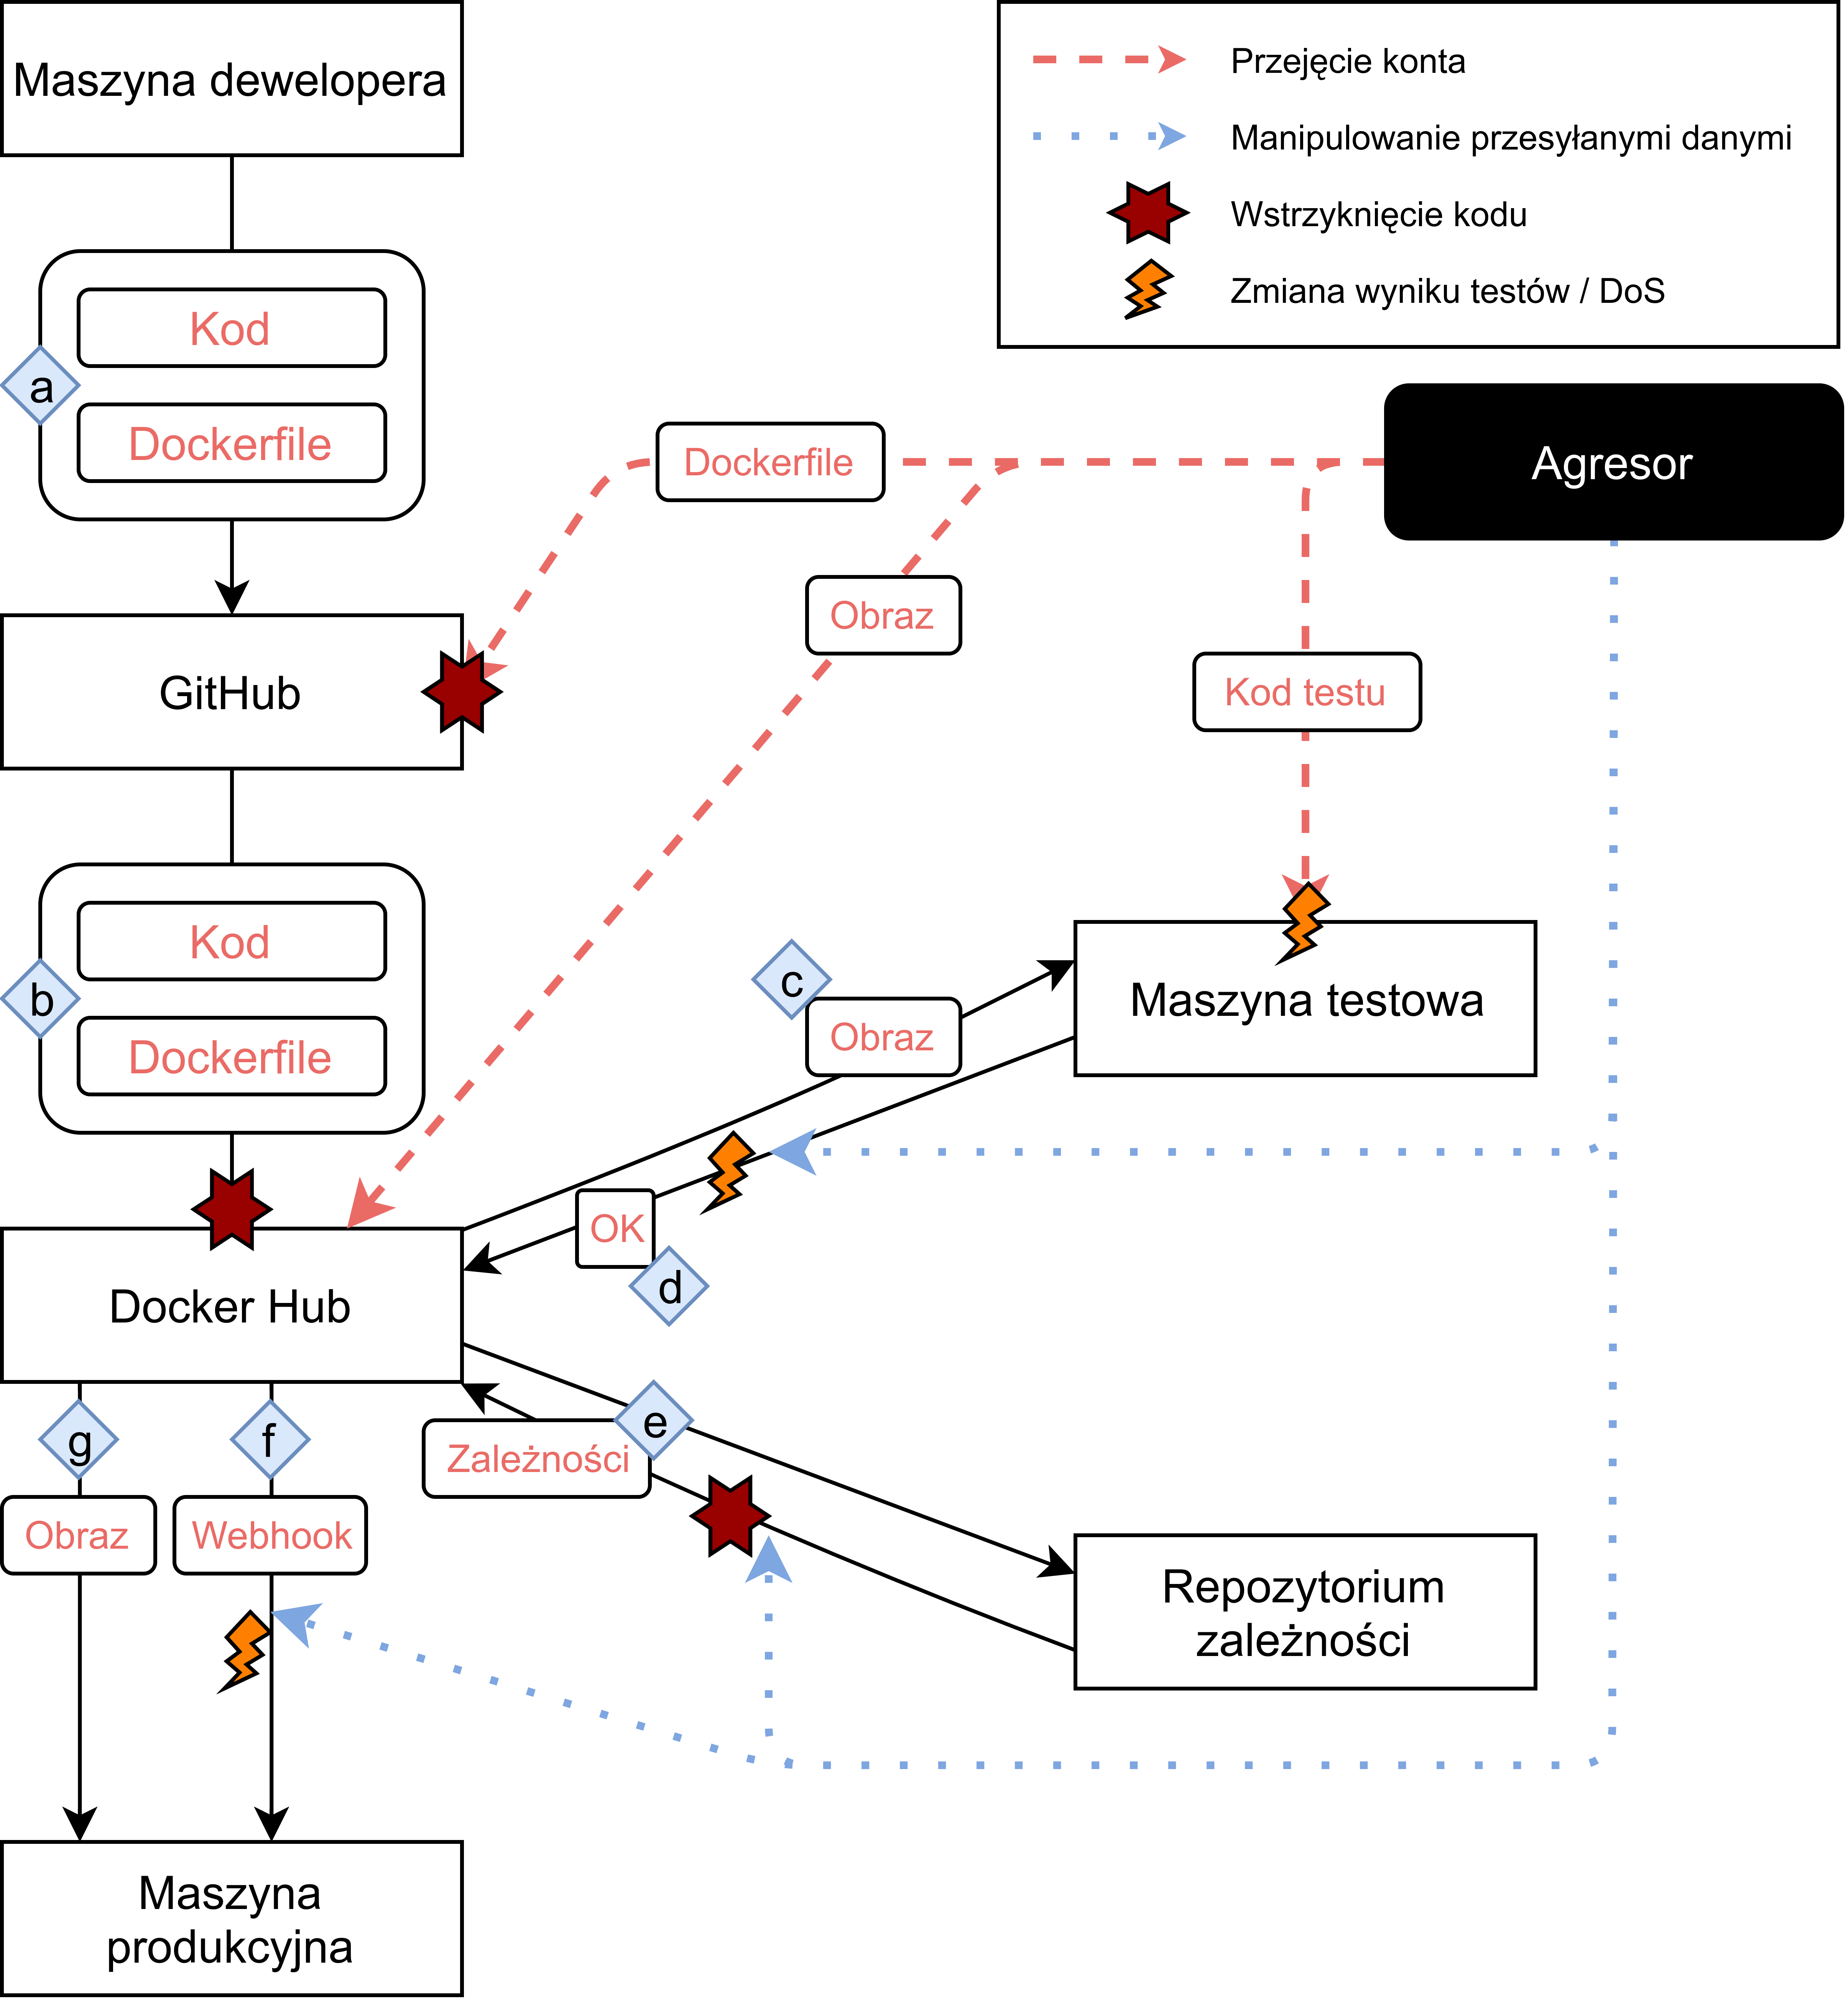
\includegraphics[width=0.9\linewidth]{images/pipeline.png}
    \caption{Rurociąg CI/CD automatycznie wdrażający kod przy użyciu usług GitHub, Docker Hub, zewnętrznej maszyny testowej i~repozytorium zależności}
    \label{fig:pipeline}
\end{figure}

Zautomatyzowane wdrożenia i~webhooki proponowane przez Docker Hub są kluczowym elementem tego procesu dystrybucji. Prowadzą do rurociągu, w~którym każdy element ma pełny dostęp do kodu ostatecznie trafiającego na produkcję. Coraz wiecej elementów jest również hostowanych w~chmurze obliczeniowej. Aby zautomatyzować to wdrożenie, Docker proponuje automatyczne budowanie obrazów w~Docker Hub, uruchamiane zdarzeniem z~zewnętrznego repozytorium kodu (np.~GitHub, BitBucket)(rys.~\ref{fig:pipeline}b). Następnie wysyłane jest żądanie HTTP do gospodarza Dockera dostępnego publicznie w~Internecie aby powiadomić go, że nowy obraz jest dostępny. Powoduje to pobranie obrazu z~rejestru i~kontener uruchamia się ponownie na nowym obrazie (rys.~\ref{fig:pipeline}f, rys.~\ref{fig:pipeline}g). W~tym typie rurociągu zatwierdzenie kodu w~repozytorium (rys.~\ref{fig:pipeline}a) zapoczątkuje budowę nowego obrazu (rys.~\ref{fig:pipeline}b), który zostanie automatycznie uruchomiony w~produkcji (rys.~\ref{fig:pipeline}f, rys.~\ref{fig:pipeline}g). Przed ostatecznym wdrożeniem można dodać opcjonalne kroki testowe, które potencjalnie mogą być uruchamianie u~jeszcze innego dostawcy (np.~GitHub Circle CI, BitBucket Pipelines). W~tym przypadku Docker Hub wysyła wpierw żądanie HTTP do maszyny testowej (rys.~\ref{fig:pipeline}c), która następnie pobiera obraz, uruchamia testy i~wysyła wyniki do Docker Hub za pomocą adresu URL wywołania zwrotnego (rys.~\ref{fig:pipeline}d). Sam proces budowania często pobiera zależności z~repozytoriów podmiotów zewnętrznych (rys.~\ref{fig:pipeline}e), czasem przez niezabezpieczony kanał (którym można manipulować). Cały potok kodu pokazano na rysunku~\ref{fig:pipeline}.

\subsection{Ataki}

W zaprezentowanej architekturze próby ataków obejmują przechwytywanie kont, manipulowanie komunikacją sieciową (w zależności od zastosowania TLS) oraz ataki z~wykorzystaniem osób wtajemniczonych (insider attack). Taka konfiguracja dodaje zewnętrzne kroki pośrednie do ścieżki, którą musi przebyć kod. Dostawcy usług mają własne systemy uwierzytelniania i~powierzchnie ataku, ogólnie zwiększając globalną powierzchnię ataku.

Przykładowo, zakładając scenariusz, w~którym skonfigurowana jest powyższa architektura agresor może uzyskać dostęp do konta w~usłudze GitHub (chociażby przy pomocy socjotechniki). Prowadzi to do wykonania złośliwego kodu na zbiorze maszyn produkcyjnych w~przeciągu kilku minut od przejęcia konta. Wyniki takiego ataku mogą być brzemienne w~skutkach jeśli na zmiany w~obrazie nasłuchuje wiele klastrów maszyn produkcyjnych. Badania pokazują, że implementacje podobnych architektur wdrażają kod z~repozytorium na maszyny produkcyjne w~czasie poniżej 5 minut \cite{CorPaulHowIsPerformanceAddressedInDevOps}.

Warto zaznaczyć, że choć zagrożenia dotyczące repozytorium kodu są niezależne od Dockera, automatyczne wdrożenie kodu do produkcji znacznie zwiększa liczbę zainfekowanych komputerów -- nawet jeśli złośliwy kod zostanie usunięty w~ciągu kolejnych kilku minut. Atak może się również odbyć na poziomie konta Docker Hub, a~konsekwencje będą takie same. Przejęcie konta nie jest nowym problemem, ale powinno być traktowane z~coraz większą troską w~związku z~mnożeniem się kont u~różnych dostawców. Ponieważ do zainfekowania kodu dochodzi na zaatakowanym komputerze, TLS jest bezużyteczny. W~rzeczywistości złośliwy kod jest „bezpiecznie” dystrybuowany przez TLS do różnych repozytoriów. Co więcej, z~powody szyfrowania komunikacji w~protokole, czuwające, ewentualne systemy IDS (Intrusion Detection System) i~IPS (Intrusion Prevention System) niczego nie wykryją. Można, co prawda, skonfigurować je do działania w~trybie man-in-the-middle i~deszyfrowania ruchu sieciowego, jednak prowadzi to do kolejnych potencjalnych luk w~zabezpieczeniach.

Ponadto, chociaż transfer kodu jest zwykle zabezpieczony za pomocą protokołu TLS, to może nie dotyczyć to wywołań API uruchamiających budowanie i~wywołań zwrotnych. Manipulowanie tymi danymi może prowadzić do błędnych wyników testów, niechcianych restartów kontenerów, itp. Co więcej, taka konfiguracja nie jest zgodna ze schematem Content Trust, ponieważ kod jest przetwarzany przez podmioty zewnętrzne znajdujące się pomiędzy deweloperem, a~środowiskiem produkcyjnym. Content Trust zapewnia środowisko, w~którym zaufany jest jeden podmiot (osoba lub organizacja, która podpisała obrazy). Podczas gdy w~niniejszym przypadku zaufanie jest podzielone na kilka podmiotów zewnętrznych, z~których każdy może narazić obrazy.

\section{Podatności wewnątrz obrazu}

\subsection{Podatności}

Podczas indeksowania Docker Hub wykazano, że 36\% oficjalnych obrazów zawiera luki CVE o~wysokim poziomie zagrożenia, a~64\% zawiera luki o~średnim lub wysokim poziomie zagrożenia. Wartości te spadają odpowiednio do 23\% i~47\% dla obrazów oznaczonych jako \textit{latest} \cite{BanyanDockerHubHighPrioritySecurityVulnerabilities}. Pomimo iż tak oznaczone obrazy są najczęściej pobieranymi w~Docker Hub, zawierają one znaczną liczbę luk w~zabezpieczeniach, w~tym niektóre z~ostatnio popularnych klas takich jak Shellshock i~Heartbleed.

Promowana przez Docker metodyka DevOps pozwala programistom samemu pakować swoje aplikacje, łącząc w~ten sposób środowiska programistyczne i~produkcyjne, a~tym samym potencjalnie wprowadzając luki. W~ostatecznej wersji obrazu Docker mogą pozostać deweloperskie wersje pakietów lub narzędzi programistycznych zwiększając tym samym jego powierzchnię ataku (np.~narzędzie do debugowania).

Stworzone obrazy często zawierają nieaktualne wersje pakietów ponieważ ich obraz podstawowy (np.~\textit{ubuntu} lub \textit{centos}) jest przestarzały lub ponieważ proces kompilacji pobiera nieaktualny kod z~jakiegoś zdalnego repozytorium. Ogrom kompilacji obrazów -- praktycznie jedna dla każdego zatwierdzenia kodu w~repozytorium projektu -- prowadzi do utrzymywania się przestarzałych obrazów, wciąż dostępnych w~repozytoriach. Z~kolei szybkie cykle programowania zwykle koncentrują się tylko i~wyłącznie na najnowszych wersjach.

\subsection{Ataki}

Wykorzystanie takich luk w~zabezpieczeniach jest istotne w~kontekście ataku z~zewnątrz. Możliwe są klasyczne metody ataków na aplikację, pod warunkiem, że kontener ujawnia punkt ataku (otwarty port sieciowy, dane wejściowe, itp.). Ponadto, obrazy zbudowane z~zewnętrznych repozytoriów kodu, tj. obrazy, które pobierają dane z~innych repozytoriów podczas procesu kompilacji (rys.~\ref{fig:pipeline}e), są zależne od tego repozytorium i~bezpieczeństwa połączenia użytego do pobrania tych danych. Te repozytoria -- nie zawsze oficjalne -- są kolejnym punktem ataku typu wstrzykiwanie kodu.

\subsection{Zapobieganie atakom}

Docker Hub korzysta z~Docker Security Scanning. Użytkownicy mogą skanować obrazy w~prywatnych repozytoriach, aby sprawdzić, czy są wolne od znanych luk w~zabezpieczeniach. Skanowanie przechodzi przez każdą warstwę obrazu, identyfikując komponenty oprogramowania i~obliczając z~nich funkcję skrótu SHA. Nastepnie są one porównywane z~bazą danych CVE w~celu uzyskania informacji o~znanych lukach bezpieczeństwa. Całkowite skanowanie trwa od 1 do 24 godzin, w~zależności od wielkości ocenianych obrazów. Udzielone wsparcie jest ograniczone ze względu na koszt usługi tylko do użytkowników Docker EE (Enterprise Edition). Co więcej, jeśli luka nie jest częścią bazy danych, skanowanie nie może jej ujawnić, przez co usługa nie reaguje na nowo pojawiające się luki \cite{DockerScanImagesForVulnerabilities}.

\section{Podatności usługi Docker}

\subsection{Podatności}

Podatności w~Docker i~\textit{libcontainer} dotyczyły głównie ataków na system gospodarza lub na bezpośrednio atakowany kontener:

\begin{itemize}
    \item uzyskanie dostępu do demona Dockera (CVE-2019-15752, CVE-2016-3697, CVE-2015-3627, CVE-2014-3499)
    \item uruchomienie arbitralnego kodu wewnątrz kontenera (CVE-2019-5736, CVE-2014-9357, CVE-2014-6407)
    \item Denial of Service (CVE-2017-14992, CVE-2016-6595)
    \item uzyskanie dodatkowych uprawnień wewnątrz kontenera (CVE-2016-8867, CVE-2014-6408)
    \item pozyskanie informacji o~systemie gospodarza (CVE-2015-3630)
    \item atak typu Directory Traversal w~systemie gospodarza (CVE-2018-15664)
\end{itemize}

Ponieważ procesy kontenerowe często działają z~uprawnieniami użytkownika \textit{root}, mają one dostęp do odczytu i~zapisu na całym systemie plików gospodarza w~momencie gdy dojdzie do ucieczki z~kontenera. W~ten sposób mogą nadpisywać pliki binarne gospodarza, co prowadzi do wykonania dowolnego kodu z~uprawnieniami administratora.

Najnowsza podatność, która pojawiła się w Dockerze w wersji 19.03.0 (CVE-2019-14271) została załatana aktualizacją do wersji 19.03.1. Aktualizacja bezpieczeństwa została opublikowana tego samego dnia, w którym pojawiły się raporty dotyczące podatności. Pokazuje to, że zespół pracujący nad Dockerem bardzo szybko reaguje na pojawiające się podatności. Jednakże, zaaplikowanie aktualizacji nadal jest zależne od użytkownika, co najczęściej powoduje znaczne wydłużenie czasu, w którym podatność jest otwarta na ataki.

\subsection{Ataki}

Oprócz przestrzeni nazw jądra, grup kontrolnych, zmniejszania uprawnień kontenerów i~ograniczeń w~montowaniu woluminów danych, obowiązkowa kontrola dostępu (ang.~Mandatory Access Control) może wymuszać ograniczenia w~przypadku nietypowego wykonywania aplikacji. Takie podejście jest widoczne w~domyślnym profilu AppArmor dla Dockera. Jednakże, wspomniana domyślna konfiguracja mogłaby być bardziej restrykcyjna. Z~reguły polityki Apparmor zwykle definiują białe listy, jawnie deklarując zasoby, do których każdy proces może uzyskać dostęp. Jednocześnie odmawiają jakiegokolwiek innego dostępu \cite{ChoiTrustworthyDesignArchitecture}. Jednak domyślny profil Dockera zapewnia kontenerom pełny dostęp do urządzeń sieciowych, systemów plików wraz z~pełnym zestawem uprawnień i~zawiera tylko niewielką listę dyrektyw odmawiających dostępu, składających się z~czarnej listy.

\section{Podatności jądra Linuxa}

Z racji iż kontenery działają na tym samym jądrze co gospodarz to są one podatne na ataki na jądro. Atak dający pełne uprawnienia użytkownika \textit{root} do kontenera może pozwolić osobie atakującej na ucieczkę z~kontenera i~narażenie systemu gospodarza (powodując naruszenie izolacji i~integralności, a~także ujawnienie danych).

\section{Ocena podatności}

\hyphenpenalty 10000
\begin{table}[ht]
    \centering
    \resizebox{\textwidth}{!}{
        \begin{tabular}{|L{4cm}|L{4cm}|L{4cm}|L{4cm}|}
            \hline
                \textbf{Kategoria podatności} &
                \textbf{Zalecany przypadek użycia} &
                \textbf{Rozpowszechniony przypadek użycia} &
                \textbf{Przypadek użycia dostawców chmurowych} \\
            \hline
                \textbf{Podatności w~konfiguracji} &
                \textbf{Umiarkowany}\newline Domyślna konfiguracja Dockera jest względnie bezpieczna. Możliwe obniżenie bezpieczeństwa konfiguracji. &
                \textbf{Bardzo wysoki}\newline Bardzo prawdopodobna niebezpieczna konfiguracja. &
                \textbf{Wysoki}\newline Kontenery w~podzie współdzielą przestrzeń nazw Network z~Kubernetes. \\
            \hline
                \textbf{Podatności w~procesie dystrybucji obrazu} &
                \textbf{Bardzo wysoki}\newline Promowana metodyka DevOps. Użycie automatyzacji na każdym kroku w~celu skrócenia cykli rozwoju oprogramowania &
                \textbf{Umiarkowany}\newline Kontery używane jako maszyny wirtualne powodując mniejszą ilość ciągłej integracji &
                \textbf{Wysoki}\newline Automatyzacja każdej warstwy w~celu ciągłego wdrażania zmian \\
            \hline
                \textbf{Podatności wewnątrz obrazu} &
                \textbf{Umiarkowany}\newline Domyślnie odsłonięta ograniczona powierzchnia ataku &
                \textbf{Bardzo wysoki}\newline Bardzo prawdopodobne użycie ciężkich obrazów z~powierzchnią ataku większą od obrazów mikroserwisów &
                \textbf{Umiarkowany}\newline W~zależności od obrazu mogą tu wystąpić przypadki użycia zalecane i~rozpowszechnione \\
            \hline
                \textbf{Podatności bezpośrednio powiązane z~Dockerem} &
                \multicolumn{3}{c|}{Podobny poziom zagrożenia we wszystkich przypadkach użycia} \\
            \hline
                \textbf{Podatności jądra Linuxa} &
                \multicolumn{3}{c|}{Podobny poziom zagrożenia we wszystkich przypadkach użycia} \\
            \hline
        \end{tabular}
    }
    \caption{Względna skala ocen poziomu zagrożenia w~trzech przypadkach użycia}
    \label{table:vulnerabilitiesAssessment}
\end{table}
\hyphenpenalty 0

Ocena poziomu zagrożenia wyjaśnionych podatności jest zależna od każdego z~przedstawionych przypadków użycia (tabela~\ref{table:vulnerabilitiesAssessment}). Zamiast koncentrować się na konkretnym przypadku zastosowania z~określoną aplikacją, przeanalizowany został ekosystem Dockera w~powiązaniu z~typowymi przypadkami użycia. Takie podejście jest również zgodne z~metodologią NIST, która definiuje kontekst jako środowisko podejmowania decyzji na bazie ryzyka i~wymiar, który należy wziąć pod uwagę podczas przeprowadzania oceny podatności na zagrożenia \cite{NISTGuideForConductingRiskAssessments}.

Ocena skupia się wyłącznie na różnicy między przypadkami użycia, przy czym wszystkie inne wymiary (zagrożenia i~środki zapobiegawcze) są równe. Szeroko rozpowszechniony przypadek użycia (używanie kontenerów jako maszyn wirtualnych) ujawnia najwięcej podatności. Co więcej, niezależnie od rozważanych przypadków użycia, podatności jądra Linuxa i~podatności bezpośrednio związane z~Dockerem mają podobny poziom zagrożenia.

\section{Alternatywy dla Dockera}

Od kilku lat, równolegle do kontenerów, rozwijane są również unikernele. Chociaż nie są one jeszcze zbyt powszechnie używane w~produkcji, rozwiązują problem izolacji poprzez uruchamianie własnego jądra, specjalnie zoptymalizowanego dla jednej aplikacji. Osiągają wydajność zbliżoną lub nawet lepszą niż kontenery, a~ich bardzo szybki rozruch pozwala na uruchomienie unikernela w~celu spełnienia określonego żądania. Dalszy rozwój technologiczny może spowodować, że w~nadchodzących latach unikernele staną się poważnym konkurentem dla kontenerów \cite{MadhavapeddyJitsu}.
